In this section, we use our own constructions based on the same edge length definition as in the previous section. The first one addresses the $n \equiv 7 \pmod{14}$ case.

\begin{definition}\label{def:1-2-3}
    Let $G$ be a graph with $7$ edges. A (1-2-3)-\emph{labeling} of $3G$ is an assignment $f$ of the integers $\{0,\dots,20\}$ to the vertices of $3G$ such that
    \begin{enumerate}
        \item $f(u) \neq f(v)$ whenever $u$ and $v$ belong to the same connected component, 
        \item[] and
        %\item there are exactly $7$ edges of length $i$ for each $i \in \{1,2,3\}$, and
       % \item if two edges $u_1v_1$ and $u_2v_2$ are of length $i$ and $u_1 \equiv v_1 \pmod7$, then $u_2 \not \equiv v_2 \pmod7.$
      %  \item when $f$ is reduced modulo $7$, there is exactly one edge of length $j$, for $j \in \{1,2,3\}$, of the form $\{i,i+j\}$ for $i \in \{0,\dots,6\}.$
        \item $$ \bigcup_{uv\in E(3G)} \{(f(u)\; \textbf{mod } 7,f(v)\; \textbf{mod } 7)\}= \bigcup_{i=0}^{6} \bigcup_{j=1}^{3} \{(i,i+j \; \textbf{mod } 7)\}.$$
    \end{enumerate}
\end{definition}
Notice that the second condition of a (1-2-3)-labeling says that $3G$ contains exactly $7$ edges of each of the lengths $1,2$, and $3$. Furthermore, no two edges of the same length have the same end labels when reduced modulo $7.$ A (1-2-3) labeling of every forest with $7$ edges with the exception of $\mathbf{T_{7}^{11}}\sqcup\mathbf{T_{2}^{1}}$ is given in Figure \ref{fig:7mod14}. This exceptional forest does not admit such a labeling and is dealt with in Section \ref{sec:star}.

\begin{thm}\label{thm:1-2-3 plus rho}
    Let $G$ be a bipartite graph with $7$ edges. If $3G$ admits a ($1$-$2$-$3$)-labeling and $G$ admits a $\rho^{+}$-labeling, then $G$ decomposes $K_{14k+7}$ for every $k\geq1.$
\end{thm}
\begin{proof}
    Let $n=14k+7$ and notice that $K_n$ has $|E(K_n)|=(7k+3)(14k+7)$ edges, which can be partitioned into $14k+7$ edges of each of the lengths in $\{1,2,\dots,7k+3\}.$  We will construct the $G$-decomposition in two steps. First, we use the 1-2-3-labeling to identify all the edges of lengths $1,2,$ and $3$ accounting for $3(2k+1)$ copies of $G$. Then, we use the $\rho^{+}$-labeling to identify edges of the remaining lengths in $7k(2k+1)$ copies of $G$. In total, the decomposition consists of $|E(K_n)|/7=(7k+3)(2k+1)$ copies of $G.$

    % Is developing by k defined?
    Let $f_1$ be a (1-2-3)-labeling of $3G$ and identify this graph as a block $B_0$. Then develop $B_0$ by 7 modulo $n$. Since the order of the development is $\frac{n}{7}=2k+1$ and there are 7 edges of each of the lengths $1,2,$ and $3$ in $B_0$, we have identified $3(2k+1)$ copies of $G$ containing all $14k+7=n$ edges of each length $1,2,$ and $3$. Notice (2) of Definition \ref{def:1-2-3} ensures no edge has been counted more than once in the development.

    Let $f_2:V(G) \rightarrow \{0,\dots,14\}$ be a $\rho^{+}$-labeling of $G$ with associated vertex partition $(A,B).$ For $i=1,2,\dots,k,$ identify blocks $B_i \cong G$ with vertex labels $\ell$ such that
    \[
    \ell(v)=
    \begin{cases}
        f_2(v), & \textrm{if } v \in A \\
        f_2(v)+3+7(i-1), & \textrm{if } v \in B
    \end{cases}
    \]
    Notice that the $i^{\textrm{th}}$ block contains exactly one edge of each length $7i-3,7i-2, \dots,$ and $ 7i+3.$ This is because every edge $ab$ has length 
    \[
    \ell(b)-\ell(a)=f_2(b)-f_2(a)+3+7(i-1)
    \]
    and $f_2(b)-f_2(a)$ is a length in $\{1,\dots,7\}.$
    Developing each block $B_i$ by 1 yields $14k+7$ copies of $G$ per block and accounts for $14k+7$ edges of each of the lengths $4,5,\dots,$ and $7k+3$.

    Since we have identified
    \[
    3(2k+1)+k(14k+7)=(7k+3)(2k+1)
    \]
    edge-disjoint copies of $G$, the proof is complete.
    % $f_2+3, f_2 + 10, \dots, f_2 + 3+7(k-1)$
    %Because $f_2$ is a $\rho$-labeling, it induces exactly one edge of each length $1,2,\dots,7.$ Further, because it is a $\rho^{+}$-labeling, fixing the labels of the $A$ vertices and increasing the set of $B$ vertices each by an integer $c$ increases the lengths by $c.$ We call this process \emph{stretching} the edges. 
\end{proof}
%%%
To address the $n \equiv 8 \pmod{14}$ case, we define the following labeling.
\begin{definition}\label{def:1-2-3-1-rot}
    Let $G$ be a graph with $7$ edges. A \emph{1-rotational $(1$-$2$-$3)$-labeling} of $4G$ is an assignment $f$ of $\{0,\dots,20\} \cup \infty$ to the vertices of $4G$ such that
    \begin{enumerate}
        \item $f(u) \neq f(v)$ whenever $u$ and $v$ belong to the same connected component, 
        \item[] and
%\item when the integer values of $f$ are reduced modulo $7$, there is exactly one edge of length $j$, for $j \in \{1,2,3\}$, of the form $\{i,i+j\}$ for $i \in \{0,\dots,6\},$ and exactly one edge of length $\infty$ of the form $\{i,\infty\}$ for $i \in \{0,\dots,6\}.$
        \item  $$ \bigcup_{uv\in E(4G)} \{(f(u)\; \textbf{mod } 7,f(v)\; \textbf{mod } 7)\}= \bigcup_{i=0}^{6} \bigcup_{j=1}^{3} \{(i,i+j \; \textbf{mod } 7), (i,\infty)\}.$$
    \end{enumerate}
\end{definition}
Notice that the second condition of a 1-rotational (1-2-3)-labeling says that $4G$ contains exactly $7$ edges of each of the lengths $1,2,3$, and $\infty$. Furthermore, no two edges of the same length have the same end labels when reduced modulo $7.$ A 1-rotational (1-2-3)-labeling of every forest with $7$ edges with the exception of $\mathbf{T_{7}^{11}}\sqcup\mathbf{T_{2}^{1}}$ is given in Figure \ref{fig:8mod14}. 

\begin{thm}\label{thm:1-2-3 1-rot plus rho}
    Let $G$ be a bipartite graph with $7$ edges. If $4G$ admits a $1$-rotational  $(1$-$2$-$3)$-labeling and $G$ admits a $\rho^{+}$-labeling, then $G$ decomposes $K_{14k+8}$ for every $k\geq1.$
\end{thm}

\begin{proof}
    Let $n=14k+8$ and notice that $K_n$ has $|E(K_n)|=(7k+4)(14k+7)$ edges, which can be partitioned into $14k+7$ edges of each of the lengths in $\{1,2,\dots,7k+3,\infty\}.$  We will construct the $G$-decomposition in two steps. First, we use the 1-rotational (1-2-3)-labeling to identify all the edges of lengths $1,2,3,$ and $\infty$ accounting for $4(2k+1)$ copies of $G$. Then, we use the $\rho^{+}$-labeling to identify edges of the remaining lengths in $7k(2k+1)$ copies of $G$. In total, the decomposition consists of $|E(K_n)|/7=(7k+4)(2k+1)$ copies of $G.$
%left off here 1/27
    Let $f_1$ be a 1-rotational (1-2-3)-labeling of $4G$ and identify this graph as a block $B_0$. Then develop $B_0$ by 7 modulo $n-1$. Since the order of the development is $\frac{n-1}{7}=2k+1$ and there are 7 edges of each of the lengths $1,2,3$ and $\infty$ in $B_0$, we have identified $4(2k+1)$ copies of $G$ containing all $14k+7=n-1$ edges of each length $1,2,3$ and $\infty$. Notice (2) of Definition \ref{def:1-2-3-1-rot} ensures no edge has been counted more than once in the development.

    Let $f_2:V(G) \rightarrow \{0,\dots,14\}$ be a $\rho^{+}$-labeling of $G$ with associated vertex partition $(A,B).$ For $i=1,2,\dots,k,$ identify blocks $B_i \cong G$ with vertex labels $\ell$ such that
    \[
    \ell(v)=
    \begin{cases}
        f_2(v), & \textrm{if } v \in A \\
        f_2(v)+3+7(i-1), & \textrm{if } v \in B
    \end{cases}
    \]
    Notice that the $i^{\textrm{th}}$ block contains exactly one edge of each length $7i-3,7i-2, \dots,$ and $ 7i+3.$ This is because every edge $ab$ has length 
    \[
    \ell(b)-\ell(a)=f_2(b)-f_2(a)+3+7(i-1)
    \]
    and $f_2(b)-f_2(a)$ is a length in $\{1,\dots,7\}.$
    Developing each block $B_i$ by 1 yields $14k+7$ copies of $G$ per block and accounts for $14k+7$ edges of each of the lengths $4,5,\dots,$ and $7k+3$.

    Since we have identified
    \[
    4(2k+1)+k(14k+7)=(7k+4)(2k+1)
    \]
    edge-disjoint copies of $G$, the proof is complete.
\end{proof}

We are now able to state the main thm of this section.
%%
\begin{thm}\label{thm:7 or 8 mod 14}
    Let $F$ be a forest with $7$ edges and $F \not \cong \mathbf{T_{7}^{11}}\sqcup\mathbf{T_{2}^{1}}$. There exists an $F$-decomposition of $K_n$ whenever $n \equiv 7 \textrm{ or } 8 \pmod{14}$ and $n \geq 21.$
\end{thm}
\begin{proof}
    If $n \equiv 7 \pmod{14},$ a (1-2-3)-labeling of $3F$ can be found in Figure \ref{fig:7mod14}. On the other hand, if $n \equiv 8 \pmod{14}$, then a 1-rotational (1-2-3)-labeling of $4F$ can be found in Figure \ref{fig:8mod14}. In either case, a $\rho^{+}$-labeling of $F$ can be found in Figure \ref{fig:sigma plus minus} (recall that a $\sigma^{+-}$-labeling is a $\rho^{+}$-labeling). The result now follows from thms \ref{thm:1-2-3 plus rho} and \ref{thm:1-2-3 1-rot plus rho}. 
\end{proof}
%%
\begin{example}
We illustrate the constructions in the previous two thms by finding an $F$-decomposition of $K_{35}$ and $K_{36}$ for the forest graph $F \cong \mathbf{T_{6}^{6}} \sqcup \mathbf{T_{3}^{1}}$. 
\newpage
\noindent Here are excerpts from the preceding tables for $\mathbf{T_{6}^{6}} \sqcup \mathbf{T_{3}^{1}}$

\begin{figure}[H]
\centering
        \scalebox{0.4}{\documentclass{standalone}
\usepackage{tikz}
\usepackage{graphicx}  % For including external images
\usepackage{standalone}  % For including standalone files
\usepackage{youngtab}  % For tables
\usepackage{array}  % For \extrarowheight support
\usepackage{amsmath}
\usepackage{longtable}  % For multi-page tables

\begin{document}
\centering
\resizebox{\textwidth}{!}{%
\begin{tabular}{|c|c|}
\hline
    Labeling Type & Labelings\\
\hline
    $\sigma^{+-}$ & $(4,1,8,5,6,7)\sqcup(10,9,11)$\\
\hline
    $7\,\pmod{14}$ & \begin{tabular}{@{}l@{}} $(0,2,1,3,4,5)\sqcup(12,11,14)$ \\
        $(4,6,8,9,5,7)\sqcup(14,12,15)$ \\
        $(0,3,1,4,5,6)\sqcup(11,8,7)$ \\
        \end{tabular}\\
\hline
    $8\,\pmod{14}$ & \begin{tabular}{@{}l@{}} $(1,2,0,3,4,5)\sqcup(11,8,\infty)$ \\
        $(2,\infty,3,4,5,6)\sqcup(12,13,15)$ \\
        $(6,7,8,4,5,\infty)\sqcup(11,12,15)$ \\
        $(11,10,8,12,13,7)\sqcup(9,6,4)$ \\ \end{tabular} \\
\hline
\end{tabular}%
}
\end{document}}
        \caption{Labelings for $\mathbf{T_{6}^{6}} \sqcup \mathbf{T_{3}^{1}}$}
        \label{fig:example chart}
\end{figure}

The $\rho^{+}$ labelings obtained by stretching the $\sigma^{+-}$ labeling are bottommost labelings in the following generating presentations and are developed by $1$.
\end{example}

%\begin{figure}[h]
%    \centering
%    \begin{tikzpicture}[scale=0.5]
%        % First standalone file
%        \node[anchor=east] (file1) at (0, 0) {\documentclass{standalone}
\usepackage{tikz}
\begin{document}
\begin{tikzpicture}[every node/.style={draw, circle, fill=black, minimum size=2pt, inner sep=0pt}]
\node[fill=black, label=above:{$v_{4}$}] (G1N1) at (90:0.5) {};
\node[fill=black, label=above left:{$v_{2}$}] (G1N0) at (90:0) {};
\node[fill=black, label=below right:{$v_{6}$}] (G1N2) at (306:0.5) {};
\node[fill=black, label=below left:{$v_{5}$}] (G1N3) at (234:0.5) {};
\node[fill=black, label=above left:{$v_{1}$}] (G1N4) at (162:0.5) {};
\node[fill=black, label=above right:{$v_{3}$}] (G1N5) at (18:0.5) {};
\draw (G1N0) -- (G1N1);
\draw (G1N0) -- (G1N2);
\draw (G1N0) -- (G1N3);
\draw (G1N0) -- (G1N4);
\draw (G1N0) -- (G1N5);
\end{tikzpicture}
\end{document}
};
%        \node[anchor=east] (Lfile1) at (0.79,-2.5) {$(4,1,8,5,6,7)$};
        % Union symbol
        
        % Second standalone file
%        \node[anchor=west] (file2) at (1, 0) {\documentclass{standalone}
\usepackage{tikz}
\begin{document}
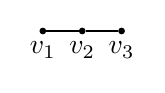
\begin{tikzpicture}[every node/.style={draw, circle, fill=black, minimum size=2pt, inner sep=0pt}]
\node[fill=black, label=below:{$v_{1}$}] (G1N1) at (6,4.5) {};
\node[fill=black, label=below:{$v_{2}$}] (G1N0) at (6.5,4.5) {};
\node[fill=black, label=below:{$v_{3}$}] (G1N2) at (7,4.5) {};
\draw (G1N0) -- (G1N1);
\draw (G1N0) -- (G1N2);
\end{tikzpicture}
\end{document}
};
%        \node[anchor=east] (Lfile1) at (4.5,-2.5) {$(10,9,11)$};
        
%    \end{tikzpicture}
%    \caption{A $\sigma^{+-}$-labeling of $\mathbf{T_{6}^{6}} \sqcup \mathbf{T_{3}^{1}}\sim (4,1,8,5,6,7)\sqcup (10,9,11)$}
%    \label{fig:union_files}
%\end{figure}
    

%%%%%%%%%%%%%%%%%%%%%%%%%%%%%%%%%%%%%%%%%%%%%%%%%%%%%%%%%%%%%%%%%%%%%%%%%%%%%%%%%%%%%%%%%%%%%%%%%
\begin{figure}[H]
    \centering
    \begin{tikzpicture}[scale=0.5]
        %G1

        \node[anchor=east] (file1) at (0, 0) {\documentclass{standalone}
\usepackage{tikz}
\begin{document}
\begin{tikzpicture}[every node/.style={draw, circle, fill=black, minimum size=2pt, inner sep=0pt}]
\node[fill=black, label=above:{$v_{4}$}] (G1N1) at (90:0.5) {};
\node[fill=black, label=above left:{$v_{2}$}] (G1N0) at (90:0) {};
\node[fill=black, label=below right:{$v_{6}$}] (G1N2) at (306:0.5) {};
\node[fill=black, label=below left:{$v_{5}$}] (G1N3) at (234:0.5) {};
\node[fill=black, label=above left:{$v_{1}$}] (G1N4) at (162:0.5) {};
\node[fill=black, label=above right:{$v_{3}$}] (G1N5) at (18:0.5) {};
\draw (G1N0) -- (G1N1);
\draw (G1N0) -- (G1N2);
\draw (G1N0) -- (G1N3);
\draw (G1N0) -- (G1N4);
\draw (G1N0) -- (G1N5);
\end{tikzpicture}
\end{document}
};
        % Union symbol
        
        % Second standalone file
        \node[anchor=west] (file2) at (0.001, -0.62) {\documentclass{standalone}
\usepackage{tikz}
\begin{document}
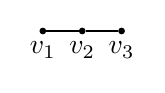
\begin{tikzpicture}[every node/.style={draw, circle, fill=black, minimum size=2pt, inner sep=0pt}]
\node[fill=black, label=below:{$v_{1}$}] (G1N1) at (6,4.5) {};
\node[fill=black, label=below:{$v_{2}$}] (G1N0) at (6.5,4.5) {};
\node[fill=black, label=below:{$v_{3}$}] (G1N2) at (7,4.5) {};
\draw (G1N0) -- (G1N1);
\draw (G1N0) -- (G1N2);
\end{tikzpicture}
\end{document}
};

    \begin{scope}[shift={(3.75,0)}]
        \draw[dashed](0,1.75)--(0,-16.75);
    \end{scope}
%%%%%%%%%%%%%%%%%%%%%%%%%%%%%%%%% second column %%%%%%%%%%%%%%%%%%%%%%%%%%%%%%%%%%%%%%%%%%%%%%%%%

    \begin{scope}[shift = {(7.75,0)}]
        
        \node[anchor=east] (file1) at (0, 0) {\documentclass{standalone}
\usepackage{tikz}
\begin{document}
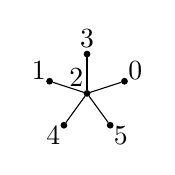
\begin{tikzpicture}[every node/.style={draw, circle, fill=black, minimum size=2pt, inner sep=0pt}]
\node[fill=black, label=above left:{$1$}] (G1N4) at (162:0.5) {};
\node[fill=black, label={[yshift=2pt]above left:{$2$}}] (G1N0) at (90:0) {};
\node[fill=black, label=above right:{$0$}] (G1N5) at (18:0.5) {};
\node[fill=black, label=above:{$3$}] (G1N1) at (90:0.5) {};
\node[fill=black, label=below left:{$4$}] (G1N3) at (234:0.5) {};
\node[fill=black, label=below right:{$5$}] (G1N2) at (306:0.5) {};

\draw (G1N0) -- (G1N1);
\draw (G1N0) -- (G1N2);
\draw (G1N0) -- (G1N3);
\draw (G1N0) -- (G1N4);
\draw (G1N0) -- (G1N5);
\end{tikzpicture}
\end{document}};
        
        \node[anchor=west] (file2) at (0.001, -0.62) {\documentclass{standalone}
\usepackage{tikz}
\begin{document}
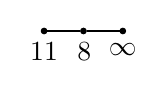
\begin{tikzpicture}[every node/.style={draw, circle, fill=black, minimum size=2pt, inner sep=0pt}]
\node[fill=black, label=below:{$11$}] (G1N1) at (6,4.5) {};
\node[fill=black, label=below:{$\;8\>$}] (G1N0) at (6.5,4.5) {};
\node[fill=black, label=below:{$\infty$}] (G1N2) at (7,4.5) {};
\draw (G1N0) -- (G1N1);
\draw (G1N0) -- (G1N2);
\end{tikzpicture}
\end{document}
};

        \draw[->] (4,0.01) -- (4,0.01) node[draw = none,midway, text=black, fill=white] {$\overset{+7}{\circlearrowright}$};
        %G2
        \node[anchor=east] (file1) at (0, -3) {\documentclass{standalone}
\usepackage{tikz}
\begin{document}
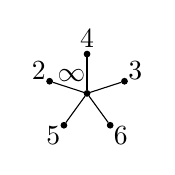
\begin{tikzpicture}[every node/.style={draw, circle, fill=black, minimum size=2pt, inner sep=0pt}]
\node[fill=black, label=above left:{$2$}] (G1N4) at (162:0.5) {};
\node[fill=black, label={[xshift=-0.85,yshift=1.5pt]above left:{$\infty$}}] (G1N0) at (90:0) {};
\node[fill=black, label=above right:{$3$}] (G1N5) at (18:0.5) {};
\node[fill=black, label=above:{$4$}] (G1N1) at (90:0.5) {};
\node[fill=black, label=below left:{$5$}] (G1N3) at (234:0.5) {};
\node[fill=black, label=below right:{$6$}] (G1N2) at (306:0.5) {};

\draw (G1N0) -- (G1N1);
\draw (G1N0) -- (G1N2);
\draw (G1N0) -- (G1N3);
\draw (G1N0) -- (G1N4);
\draw (G1N0) -- (G1N5);
\end{tikzpicture}
\end{document}};
        
        \node[anchor=west] (file2) at (0.001, -3.62) {\documentclass{standalone}
\usepackage{tikz}
\begin{document}
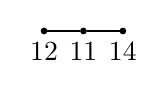
\begin{tikzpicture}[every node/.style={draw, circle, fill=black, minimum size=2pt, inner sep=0pt}]
\node[fill=black, label=below:{$12$}] (G1N1) at (6,4.5) {};
\node[fill=black, label=below:{$11$}] (G1N0) at (6.5,4.5) {};
\node[fill=black, label=below:{$14$}] (G1N2) at (7,4.5) {};
\draw (G1N0) -- (G1N1);
\draw (G1N0) -- (G1N2);
\end{tikzpicture}
\end{document}
};

        \draw[->] (4,-3.01) -- (4,-3.01) node[draw = none,midway, text=black, fill=white] {$\overset{+7}{\circlearrowright}$};
        %G3
        \node[anchor=east] (file1) at (0, -6) {\documentclass{standalone}
\usepackage{tikz}
\begin{document}
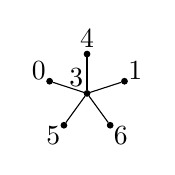
\begin{tikzpicture}[every node/.style={draw, circle, fill=black, minimum size=2pt, inner sep=0pt}]
\node[fill=black, label=above left:{$0$}] (G1N4) at (162:0.5) {};
\node[fill=black, label={[yshift=2pt]above left:{$3$}}] (G1N0) at (90:0) {};
\node[fill=black, label=above right:{$1$}] (G1N5) at (18:0.5) {};
\node[fill=black, label=above:{$4$}] (G1N1) at (90:0.5) {};
\node[fill=black, label=below left:{$5$}] (G1N3) at (234:0.5) {};
\node[fill=black, label=below right:{$6$}] (G1N2) at (306:0.5) {};
\draw (G1N0) -- (G1N1);
\draw (G1N0) -- (G1N2);
\draw (G1N0) -- (G1N3);
\draw (G1N0) -- (G1N4);
\draw (G1N0) -- (G1N5);
\end{tikzpicture}
\end{document}
};
        
        \node[anchor=west] (file2) at (0.001, -6.62) {\documentclass{standalone}
\usepackage{tikz}
\begin{document}
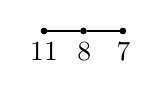
\begin{tikzpicture}[every node/.style={draw, circle, fill=black, minimum size=2pt, inner sep=0pt}]
\node[fill=black, label=below:{$11$}] (G1N1) at (6,4.5) {};
\node[fill=black, label=below:{$\;8\>$}] (G1N0) at (6.5,4.5) {};
\node[fill=black, label=below:{$\;7\>$}] (G1N2) at (7,4.5) {};
\draw (G1N0) -- (G1N1);
\draw (G1N0) -- (G1N2);
\end{tikzpicture}
\end{document}
};

        \draw[->] (4,-6.01) -- (4,-6.01) node[draw = none,midway, text=black, fill=white] {$\overset{+7}{\circlearrowright}$};
        %G4
        \node[anchor=east] (file1) at (0.246, -9) {\documentclass{standalone}
\usepackage{tikz}
\begin{document}
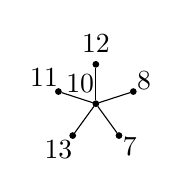
\begin{tikzpicture}[every node/.style={draw, circle, fill=black, minimum size=2pt, inner sep=0pt}]
\node[fill=black, label=above left:{$11$}] (G1N4) at (162:0.5) {};
\node[fill=black, label={[xshift=-0.5,yshift=2pt]above left:{$10$}}] (G1N0) at (90:0) {};
\node[fill=black, label=above right:{$8$}] (G1N5) at (18:0.5) {};
\node[fill=black, label=above:{$12$}] (G1N1) at (90:0.5) {};
\node[fill=black, label=below left:{$13$}] (G1N3) at (234:0.5) {};
\node[fill=black, label=below right:{$7$}] (G1N2) at (306:0.5) {};

\draw (G1N0) -- (G1N1);
\draw (G1N0) -- (G1N2);
\draw (G1N0) -- (G1N3);
\draw (G1N0) -- (G1N4);
\draw (G1N0) -- (G1N5);
\end{tikzpicture}
\end{document}};
        
        \node[anchor=west] (file2) at (0.001, -9.62) {\documentclass{standalone}
\usepackage{tikz}
\begin{document}
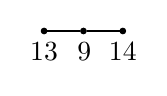
\begin{tikzpicture}[every node/.style={draw, circle, fill=black, minimum size=2pt, inner sep=0pt}]
\node[fill=black, label=below:{$13$}] (G1N1) at (6,4.5) {};
\node[fill=black, label=below:{$\;9\>$}] (G1N0) at (6.5,4.5) {};
\node[fill=black, label=below:{$14$}] (G1N2) at (7,4.5) {};
\draw (G1N0) -- (G1N1);
\draw (G1N0) -- (G1N2);
\end{tikzpicture}
\end{document}
};

        \draw[->] (4,-9.01) -- (4,-9.01) node[draw = none,midway, text=black, fill=white] {$\overset{+1}{\circlearrowright}$};

        %G5
        \node[anchor=east] (file1) at (0.246, -12) {\documentclass{standalone}
\usepackage{tikz}
\begin{document}
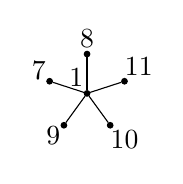
\begin{tikzpicture}[every node/.style={draw, circle, fill=black, minimum size=2pt, inner sep=0pt}]
\node[fill=black, label=above left:{$7$}] (G1N4) at (162:0.5) {};
\node[fill=black, label={[yshift=2pt]above left:{$1$}}] (G1N0) at (90:0) {};
\node[fill=black, label=above right:{$11$}] (G1N5) at (18:0.5) {};
\node[fill=black, label=above:{$8$}] (G1N1) at (90:0.5) {};
\node[fill=black, label=below left:{$9$}] (G1N3) at (234:0.5) {};
\node[fill=black, label=below right:{$10$}] (G1N2) at (306:0.5) {};
\draw (G1N0) -- (G1N1);
\draw (G1N0) -- (G1N2);
\draw (G1N0) -- (G1N3);
\draw (G1N0) -- (G1N4);
\draw (G1N0) -- (G1N5);
\end{tikzpicture}
\end{document}};
        
        \node[anchor=west] (file2) at (0.001, -12.62) {\documentclass{standalone}
\usepackage{tikz}
\begin{document}
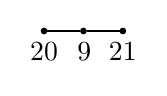
\begin{tikzpicture}[every node/.style={draw, circle, fill=black, minimum size=2pt, inner sep=0pt}]
\node[fill=black, label=below:{$20$}] (G1N1) at (6,4.5) {};
\node[fill=black, label=below:{$\;9\>$}] (G1N0) at (6.5,4.5) {};
\node[fill=black, label=below:{$21$}] (G1N2) at (7,4.5) {};
\draw (G1N0) -- (G1N1);
\draw (G1N0) -- (G1N2);
\end{tikzpicture}
\end{document}};

        \draw[->] (4,-12.01) -- (4,-12.01) node[draw = none,midway, text=black, fill=white] {$\overset{+1}{\circlearrowright}$};
        \end{scope}
        
    \begin{scope}[shift={(12.9555,0)}]
        \draw[dashed](0,1.75)--(0,-16.75);
    \end{scope}
%%%%%%%%%%%%%%%%%%%%%%%%%%%%%%%%% third column %%%%%%%%%%%%%%%%%%%%%%%%%%%%%%%%%%%%%%%%%%%%%%%%%%
    \begin{scope}[shift={(17,0)}]

        %G1
        \node[anchor=east] (file1) at (0, 0) {\documentclass{standalone}
\usepackage{tikz}
\begin{document}
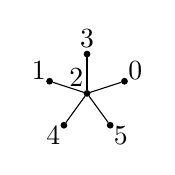
\begin{tikzpicture}[every node/.style={draw, circle, fill=black, minimum size=2pt, inner sep=0pt}]
\node[fill=black, label=above left:{$1$}] (G1N4) at (162:0.5) {};
\node[fill=black, label={[yshift=2pt]above left:{$2$}}] (G1N0) at (90:0) {};
\node[fill=black, label=above right:{$0$}] (G1N5) at (18:0.5) {};
\node[fill=black, label=above:{$3$}] (G1N1) at (90:0.5) {};
\node[fill=black, label=below left:{$4$}] (G1N3) at (234:0.5) {};
\node[fill=black, label=below right:{$5$}] (G1N2) at (306:0.5) {};

\draw (G1N0) -- (G1N1);
\draw (G1N0) -- (G1N2);
\draw (G1N0) -- (G1N3);
\draw (G1N0) -- (G1N4);
\draw (G1N0) -- (G1N5);
\end{tikzpicture}
\end{document}};
        
        \node[anchor=west] (file2) at (0.001, -0.62) {\documentclass{standalone}
\usepackage{tikz}
\begin{document}
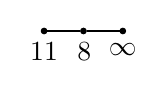
\begin{tikzpicture}[every node/.style={draw, circle, fill=black, minimum size=2pt, inner sep=0pt}]
\node[fill=black, label=below:{$11$}] (G1N1) at (6,4.5) {};
\node[fill=black, label=below:{$\;8\>$}] (G1N0) at (6.5,4.5) {};
\node[fill=black, label=below:{$\infty$}] (G1N2) at (7,4.5) {};
\draw (G1N0) -- (G1N1);
\draw (G1N0) -- (G1N2);
\end{tikzpicture}
\end{document}
};

        \draw[->] (4,0.01) -- (4,0.01) node[draw = none,midway, text=black, fill=white] {$\overset{+7}{\circlearrowright}$};
        %G2
        \node[anchor=east] (file1) at (0, -3) {\documentclass{standalone}
\usepackage{tikz}
\begin{document}
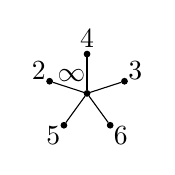
\begin{tikzpicture}[every node/.style={draw, circle, fill=black, minimum size=2pt, inner sep=0pt}]
\node[fill=black, label=above left:{$2$}] (G1N4) at (162:0.5) {};
\node[fill=black, label={[xshift=-0.85,yshift=1.5pt]above left:{$\infty$}}] (G1N0) at (90:0) {};
\node[fill=black, label=above right:{$3$}] (G1N5) at (18:0.5) {};
\node[fill=black, label=above:{$4$}] (G1N1) at (90:0.5) {};
\node[fill=black, label=below left:{$5$}] (G1N3) at (234:0.5) {};
\node[fill=black, label=below right:{$6$}] (G1N2) at (306:0.5) {};

\draw (G1N0) -- (G1N1);
\draw (G1N0) -- (G1N2);
\draw (G1N0) -- (G1N3);
\draw (G1N0) -- (G1N4);
\draw (G1N0) -- (G1N5);
\end{tikzpicture}
\end{document}};
        
        \node[anchor=west] (file2) at (0.001, -3.62) {\documentclass{standalone}
\usepackage{tikz}
\begin{document}
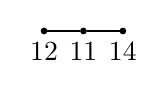
\begin{tikzpicture}[every node/.style={draw, circle, fill=black, minimum size=2pt, inner sep=0pt}]
\node[fill=black, label=below:{$12$}] (G1N1) at (6,4.5) {};
\node[fill=black, label=below:{$11$}] (G1N0) at (6.5,4.5) {};
\node[fill=black, label=below:{$14$}] (G1N2) at (7,4.5) {};
\draw (G1N0) -- (G1N1);
\draw (G1N0) -- (G1N2);
\end{tikzpicture}
\end{document}
};

        \draw[->] (4,-3.01) -- (4,-3.01) node[draw = none,midway, text=black, fill=white] {$\overset{+7}{\circlearrowright}$};
        %G3
        \node[anchor=east] (file1) at (0, -6) {\documentclass{standalone}
\usepackage{tikz}
\begin{document}
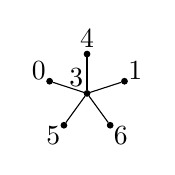
\begin{tikzpicture}[every node/.style={draw, circle, fill=black, minimum size=2pt, inner sep=0pt}]
\node[fill=black, label=above left:{$0$}] (G1N4) at (162:0.5) {};
\node[fill=black, label={[yshift=2pt]above left:{$3$}}] (G1N0) at (90:0) {};
\node[fill=black, label=above right:{$1$}] (G1N5) at (18:0.5) {};
\node[fill=black, label=above:{$4$}] (G1N1) at (90:0.5) {};
\node[fill=black, label=below left:{$5$}] (G1N3) at (234:0.5) {};
\node[fill=black, label=below right:{$6$}] (G1N2) at (306:0.5) {};
\draw (G1N0) -- (G1N1);
\draw (G1N0) -- (G1N2);
\draw (G1N0) -- (G1N3);
\draw (G1N0) -- (G1N4);
\draw (G1N0) -- (G1N5);
\end{tikzpicture}
\end{document}
};
        
        \node[anchor=west] (file2) at (0.001, -6.62) {\documentclass{standalone}
\usepackage{tikz}
\begin{document}
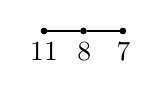
\begin{tikzpicture}[every node/.style={draw, circle, fill=black, minimum size=2pt, inner sep=0pt}]
\node[fill=black, label=below:{$11$}] (G1N1) at (6,4.5) {};
\node[fill=black, label=below:{$\;8\>$}] (G1N0) at (6.5,4.5) {};
\node[fill=black, label=below:{$\;7\>$}] (G1N2) at (7,4.5) {};
\draw (G1N0) -- (G1N1);
\draw (G1N0) -- (G1N2);
\end{tikzpicture}
\end{document}
};

        \draw[->] (4,-6.01) -- (4,-6.01) node[draw = none,midway, text=black, fill=white] {$\overset{+7}{\circlearrowright}$};
        %G4
        \node[anchor=east] (file1) at (0, -9) {\documentclass{standalone}
\usepackage{tikz}
\begin{document}
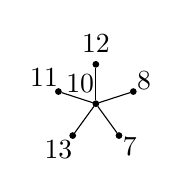
\begin{tikzpicture}[every node/.style={draw, circle, fill=black, minimum size=2pt, inner sep=0pt}]
\node[fill=black, label=above left:{$11$}] (G1N4) at (162:0.5) {};
\node[fill=black, label={[xshift=-0.5,yshift=2pt]above left:{$10$}}] (G1N0) at (90:0) {};
\node[fill=black, label=above right:{$8$}] (G1N5) at (18:0.5) {};
\node[fill=black, label=above:{$12$}] (G1N1) at (90:0.5) {};
\node[fill=black, label=below left:{$13$}] (G1N3) at (234:0.5) {};
\node[fill=black, label=below right:{$7$}] (G1N2) at (306:0.5) {};

\draw (G1N0) -- (G1N1);
\draw (G1N0) -- (G1N2);
\draw (G1N0) -- (G1N3);
\draw (G1N0) -- (G1N4);
\draw (G1N0) -- (G1N5);
\end{tikzpicture}
\end{document}};
        
        \node[anchor=west] (file2) at (0.001, -9.62) {\documentclass{standalone}
\usepackage{tikz}
\begin{document}
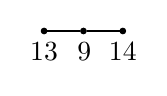
\begin{tikzpicture}[every node/.style={draw, circle, fill=black, minimum size=2pt, inner sep=0pt}]
\node[fill=black, label=below:{$13$}] (G1N1) at (6,4.5) {};
\node[fill=black, label=below:{$\;9\>$}] (G1N0) at (6.5,4.5) {};
\node[fill=black, label=below:{$14$}] (G1N2) at (7,4.5) {};
\draw (G1N0) -- (G1N1);
\draw (G1N0) -- (G1N2);
\end{tikzpicture}
\end{document}
};

        \draw[->] (4,-9.01) -- (4,-9.01) node[draw = none,midway, text=black, fill=white] {$\overset{+7}{\circlearrowright}$};
        
        %G5
        \node[anchor=east] (file1) at (0.246, -12) {\documentclass{standalone}
\usepackage{tikz}
\begin{document}
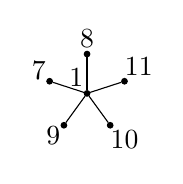
\begin{tikzpicture}[every node/.style={draw, circle, fill=black, minimum size=2pt, inner sep=0pt}]
\node[fill=black, label=above left:{$7$}] (G1N4) at (162:0.5) {};
\node[fill=black, label={[yshift=2pt]above left:{$1$}}] (G1N0) at (90:0) {};
\node[fill=black, label=above right:{$11$}] (G1N5) at (18:0.5) {};
\node[fill=black, label=above:{$8$}] (G1N1) at (90:0.5) {};
\node[fill=black, label=below left:{$9$}] (G1N3) at (234:0.5) {};
\node[fill=black, label=below right:{$10$}] (G1N2) at (306:0.5) {};
\draw (G1N0) -- (G1N1);
\draw (G1N0) -- (G1N2);
\draw (G1N0) -- (G1N3);
\draw (G1N0) -- (G1N4);
\draw (G1N0) -- (G1N5);
\end{tikzpicture}
\end{document}};
        
        \node[anchor=west] (file2) at (0.001, -12.62) {\documentclass{standalone}
\usepackage{tikz}
\begin{document}
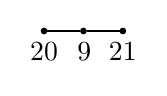
\begin{tikzpicture}[every node/.style={draw, circle, fill=black, minimum size=2pt, inner sep=0pt}]
\node[fill=black, label=below:{$20$}] (G1N1) at (6,4.5) {};
\node[fill=black, label=below:{$\;9\>$}] (G1N0) at (6.5,4.5) {};
\node[fill=black, label=below:{$21$}] (G1N2) at (7,4.5) {};
\draw (G1N0) -- (G1N1);
\draw (G1N0) -- (G1N2);
\end{tikzpicture}
\end{document}};

        \draw[->] (4,-12.01) -- (4,-12.01) node[draw = none,midway, text=black, fill=white] {$\overset{+1}{\circlearrowright}$};

        %G6
        \node[anchor=east] (file1) at (0.246, -15) {\documentclass{standalone}
\usepackage{tikz}
\begin{document}
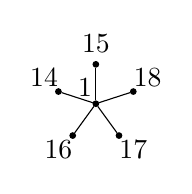
\begin{tikzpicture}[every node/.style={draw, circle, fill=black, minimum size=2pt, inner sep=0pt}]
\node[fill=black, label=above left:{$14$}] (G1N4) at (162:0.5) {};
\node[fill=black, label={[yshift=2pt]above left:{$1$}}] (G1N0) at (90:0) {};
\node[fill=black, label=above right:{$18$}] (G1N5) at (18:0.5) {};
\node[fill=black, label=above:{$15$}] (G1N1) at (90:0.5) {};
\node[fill=black, label=below left:{$16$}] (G1N3) at (234:0.5) {};
\node[fill=black, label=below right:{$17$}] (G1N2) at (306:0.5) {};
\draw (G1N0) -- (G1N1);
\draw (G1N0) -- (G1N2);
\draw (G1N0) -- (G1N3);
\draw (G1N0) -- (G1N4);
\draw (G1N0) -- (G1N5);
\end{tikzpicture}
\end{document}
};
        
        \node[anchor=west] (file2) at (0.001, -15.62) {\documentclass{standalone}
\usepackage{tikz}
\begin{document}
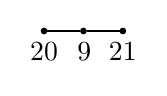
\begin{tikzpicture}[every node/.style={draw, circle, fill=black, minimum size=2pt, inner sep=0pt}]
\node[fill=black, label=below:{$20$}] (G1N1) at (6,4.5) {};
\node[fill=black, label=below:{$\;9\>$}] (G1N0) at (6.5,4.5) {};
\node[fill=black, label=below:{$21$}] (G1N2) at (7,4.5) {};
\draw (G1N0) -- (G1N1);
\draw (G1N0) -- (G1N2);
\end{tikzpicture}
\end{document}};

        \draw[->] (4,-15.01) -- (4,-15.01) node[draw = none,midway, text=black, fill=white] {$\overset{+1}{\circlearrowright}$};

    \end{scope}
    \end{tikzpicture}
    \caption{A $\sigma^{+-}$-labeling of $F \cong\mathbf{T_{6}^{6}} \sqcup \mathbf{T_{3}^{1}}$ (left) and generating presentations for the $F$-decomposition of $K_{n}$ where $n=35$ (middle) and $n=36$ (right)}
    \label{fig:7mod14example}
\end{figure}